%\documentstyle[10pt,twoside]{article}
%\documentstyle[twoside]{article}
\documentclass[twoside]{article}
\setlength{\oddsidemargin}{0.25 in}
\setlength{\evensidemargin}{-0.25 in}
\setlength{\topmargin}{-0.6 in}
\setlength{\textwidth}{6.5 in}
\setlength{\textheight}{8.5 in}
\setlength{\headsep}{0.75 in}
\setlength{\parindent}{0 in}
\setlength{\parskip}{0.1 in}

\usepackage{graphicx}
\usepackage{changepage}
\graphicspath{ {images/} }
\usepackage{url}
\usepackage{amsmath}

%
% The following commands sets up the lecnum (lecture number)
% counter and make various numbering schemes work relative
% to the lecture number.
%
\newcounter{lecnum}
\renewcommand{\thepage}{\thelecnum-\arabic{page}}
\renewcommand{\thesection}{\thelecnum.\arabic{section}}
\renewcommand{\theequation}{\thelecnum.\arabic{equation}}
\renewcommand{\thefigure}{\thelecnum.\arabic{figure}}
\renewcommand{\thetable}{\thelecnum.\arabic{table}}
\newcommand{\dnl}{\mbox{}\par}

%
% The following macro is used to generate the header.
%
\newcommand{\lecture}[4]{
   \pagestyle{myheadings}
   \thispagestyle{plain}
   \newpage
   \setcounter{lecnum}{#1}
   \setcounter{page}{1}
   \noindent
   \begin{center}
   \framebox{
      \vbox{\vspace{2mm}
    \hbox to 6.28in { {\bf CMPSCI~677~~~Operating Systems
                        \hfill Spring 2019} }
       \vspace{4mm}
       \hbox to 6.28in { {\Large \hfill Lecture #1: #2  \hfill} }
       \vspace{2mm}
       \hbox to 6.28in { {\it Lecturer: #3 \hfill Scribe: #4} }
      \vspace{2mm}}
   }
   \end{center}
   \markboth{Lecture #1: #2}{Lecture #1: #2}
   \vspace*{4mm}
}

%
% Convention for citations is authors' initials followed by the year.
% For example, to cite a paper by Leighton and Maggs you would type
% \cite{LM89}, and to cite a paper by Strassen you would type \cite{S69}.
% (To avoid bibliography problems, for now we redefine the \cite command.)
%
\renewcommand{\cite}[1]{[#1]}

% \input{epsf}

%Use this command for a figure; it puts a figure in wherever you want it.
%usage: \fig{NUMBER}{FIGURE-SIZE}{CAPTION}{FILENAME}
\newcommand{\fig}[4]{
            %\vspace{0.2 in}
            \centerline{\includegraphics[scale=#2]{#4}}
            \begin{center}
            Figure \thelecnum.#1:~#3
            \end{center}
    }

% Use these for theorems, lemmas, proofs, etc.
\newtheorem{theorem}{Theorem}[lecnum]
\newtheorem{lemma}[theorem]{Lemma}
\newtheorem{proposition}[theorem]{Proposition}
\newtheorem{claim}[theorem]{Claim}
\newtheorem{corollary}[theorem]{Corollary}
\newtheorem{definition}[theorem]{Definition}
\newenvironment{proof}{{\bf Proof:}}{\hfill\rule{2mm}{2mm}}

% Some useful equation alignment commands, borrowed from TeX
\makeatletter
\def\eqalign#1{\,\vcenter{\openup\jot\m@th
  \ialign{\strut\hfil$\displaystyle{##}$&$\displaystyle{{}##}$\hfil
      \crcr#1\crcr}}\,}
\def\eqalignno#1{\displ@y \tabskip\@centering
  \halign to\displaywidth{\hfil$\displaystyle{##}$\tabskip\z@skip
    &$\displaystyle{{}##}$\hfil\tabskip\@centering
    &\llap{$##$}\tabskip\z@skip\crcr
    #1\crcr}}
\def\leqalignno#1{\displ@y \tabskip\@centering
  \halign to\displaywidth{\hfil$\displaystyle{##}$\tabskip\z@skip
    &$\displaystyle{{}##}$\hfil\tabskip\@centering
    &\kern-\displaywidth\rlap{$##$}\tabskip\displaywidth\crcr
    #1\crcr}}
\makeatother

% **** IF YOU WANT TO DEFINE ADDITIONAL MACROS FOR YOURSELF, PUT THEM HERE:



% Some general latex examples and examples making use of the
% macros follow.

\begin{document}

% FILL IN THE RIGHT INFO.
% \lecture{**LECTURE-NUMBER**}{**DATE**}{**LECTURER**}{**SCRIBE**}
\lecture{18}{April 1}{Prashant Shenoy}{\textbf{Chen Qu (2019), Sheshera Mysore (2017)}}

This lecture spoke about the implementation paradigms for consistency in replication and then moved to the next larger topic of fault tolerance.
\section{Lecture 17 Cont'd}
\textbf{Removing Data}:

Deletion of data items is harder than it looks in epidemic protocols.

suppose you have a file that is replicated on multiple machines. You delete it on one of the replicas. That replica contacts another server and they try to compare the data items. You'll see that the first server where the file was deleted will look like it has one file missing, which is present on another server. If you do pair-wise exchange, that file that you deleted will reappear because you pull that file thinking it's a new data item you've never seen before. So deleting any data without leaving any trace of the deletion is problematic in epidemic protocols because pair-wise exchanges require you to do a diff and you get either new data items or a modified version you've never seen before.

To deal with this issue, we have to keep state of what's been deleted. That's called death certificates. Every time you delete a file, you can delete the file itself but keep a record saying that such a file existed and it was deleted. That's the data update to that file. When you do pair-wise exchange, you would spread that death-certificate, which means it will trigger deletes on other replicas and they will keep the death certificate a record of a file deletion.

The issue of this is that over a long period of time, there will be a log file deleted so you will have a lot of death certificate in the system. This is resource consuming. So once in a while, you need to go back and clean very old death certificates. You only delete the death certificates when you have high confidence that all replica copies of that file were deleted.

\section{Implementing Consistency Models}

There are two methods to implement consistency mechanisms.

\begin{enumerate}
\item \textbf{Primary based protocols}  
  These work by designating a primary replica for each data item. Different replicas could be primaries for different data items. The updates of a file are always sent to the primary first and the primary tracks the most recent version of the file. Then the primary propagates all updates (writes) to other replicas.  Within primary based protocols there are two variants:
  \begin{description}
   \item [Remote write protocols:] In the first slide for Remote-Write Protocols, there is no replication thus no consistency issues. In the second slide, there is a primary server for item x. Here all writes to a file must be forwarded to a fixed primary server responsible for the file. This primary in turn updates all replicas of the data and sends an acknowledgement to the blocked client process making the write. Since write are only allowed through a primary the order in which writes were made is straightforward to determine which ensures sequential consistency.
   \item [Local write protocols:] Here a client wishing to write to a replicated file is allowed to do so by migrating the primary copy of a file to a replica server which is local to the client. The client may therefore make many write operations locally while updates to other replicas are carried out asynchronously. There is only one primary at anytime.
  \end{description}
  Both these variants of primary based protocols are implemented in NFS.
  
  \textit{2019 QA\\
  Q: Do we need to broadcast to all clients of the fact that the primary has been moved?\\
  A: Typically no. But it depends on the system. Ideally, we don't want to let the client know where the primary is. The system deals with it internally.\\
  Follow-up Q: I actually mean that if the servers need to know who the primary is.\\
  A: Yes.\\
}

\item \textbf{Replicated write protocols}
  In this class of protocols, there is no single primary per file and any replica can be updated by a client. This framework makes it harder to achieve consistency. For the set of writes made by the client it becomes challenging to establish the correct order in which the writes were made. Replicated write protocols are implemented most often by means of quorum-based protocols. These are a class of protocols which guarantee consistency by means of voting between clients. These are discussed next.
\end{enumerate}

\subsection{Gifford's Quorum-Based Protocol}
The idea in Quorum based protocols is for a client wishing to perform a read or a write to acquire the permission of multiple servers for either of those operations. In a system with $N$ replicas of a file if a client wishes to read a file it can only read a file if $N_R$ (the read quorum) of these replica nodes agree on the version of the file (in case of disagreement a different quorum must be assembled and a re-attempt must be made). To write a file, the client must do so by writing to at-least $N_W$ (the write quorum) replicas. The system of voting can ensure consistency if the following constraints on the read and write quorums are established:
\begin{align}
  N_{R} + N_{W} > N\\ 
  N_{W} > N / 2
\end{align}

This set of constraints ensures that one write quorum node is always present in the read quorum. Therefore a read request would never be made to a subset of servers and yield the older version file since the one node common to both would disagree on the file version. The second constraint also makes sure that there is only one ongoing write made to a file at any given time. Different values of $N_R$ and $N_W$ are illustrated in Figure \ref{fig:voting}

\begin{figure}
\begin{center}
   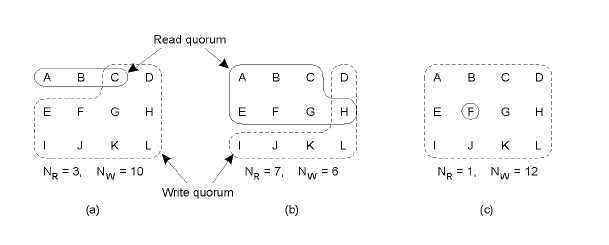
\includegraphics[width=0.8\textwidth]{quorum.png}
   \caption{Different settings of $N_{R}$ and $N_{W}$.}
   \label{fig:voting}
 \end{center}
\end{figure}

\textit{Q: Should all write quorum nodes be up to date before a new write is made?\\
  A: Here we assume that a write re-writes the entire file. In case parts of the file were being updated this would be necessary.\\
  Q: Should all writes happen atomically?\\
  A: This is an implementation detail, but yes. All the writes must acknowledge with the client before the write is committed.\\
  Q: Can you read from the read quorum and just select the maximum version file?\\
  A: Yes. But you want them to agree.
}

  \textit{2019 QA\\
  Q: If you have a lot of replications (e.g. thousands), and you have those two conditions, would it be very slow?\\
  A: That's indeed the case. Ensuring consistency can be expensive.\\
  }

\section{Replica Management}
Some of the design choices involved in deciding how to replicate resources are:
\begin{itemize}
 \item How many copies do we want? The degree of three can give reasonable guarantees. This degree depends on what we want to achieve.
 \item You want to place replicated resources closer to users.
 \item Can you cache content instead of replicating entire resources?
 \item Should replication be client initiated or server initiated?
\end{itemize}

\textit{Q: Is caching a form of client initiated replication?\\
  A: Yes, but client initiated could be broader than just caching of content, it could even be replication of computation. In case of gaming applications client demand for the game in a certain location may lead to the addition of servers closer to the clients, this would be client initiated replication as well.}

\section{Content Distribution}
A set of caches that replicate contents. Dynamic caching starts fetching contents on the fly when users start accessing them. When we have high degree of replication, how do we deal with consistency. Will you send the new data to caches or do you just tell them to throw out out-dated data (update vs. invalidate). 

  \textit{2019 QA\\
  Q: Does the cache contains information that where a certain resource is always valid (i.e. it's ``home'')?\\
  A: We need to keep additional state for consistency.\\
  }

% 
% \begin{adjustwidth}{1cm}{1cm}
%   \begin{description}
%     \item [Safety] Something bad will never happen
%     \item [Liveness] Something good will eventually happen
%   \end{description}
% \end{adjustwidth}

\section{Fault Tolerance}

Fault tolerant refers to ability of systems to work in spite of system failures. This is important in large distributed since a larger number of components imply a larger number of failures, which means the probability of at least one failure is high. Failures themselves could be hardware crashes or software bugs (which exist because most software systems are shipped when they are ``good enough'').

A perspective of fault tolerance: computing systems are not very reliable. Some computing systems are mission critical, such as auto-pilot on a car or smart TV. We cannot/don't want to simply reboot these systems when they fail. So fault tolerance is important. In addition, we need to make computing systems more reliable, especially for online-banking, etc.

A system's \textit{dependability} is evaluated based on:
\begin{itemize}
  \item Availability: The percentage of time for which a system is available. Gold standard is that of the ``five nines'' i.e a system is available 99.999\% of the time. This translates to a few minutes of down-time per year.
  \item Reliability: System must run continuously without failure.
  \item Safety: System failures should not compromise safety of client systems and lead to catastrophic failures.
  \item Maintainability: Systems failures should be easy to fix.
\end{itemize}

Basic concepts:
\begin{itemize}
    \item Transient faults: when the system is running, it sees occasional errors but continues to run. The errors come and go, but do not bring the system down.
    \item intermittent faults: the system may die occasionally but if you restart it, it comes back up.
    \item Permanent faults: the system is dead and not coming back up.
\end{itemize}

\subsection{Failure Models}
\begin{figure}
\begin{center}
   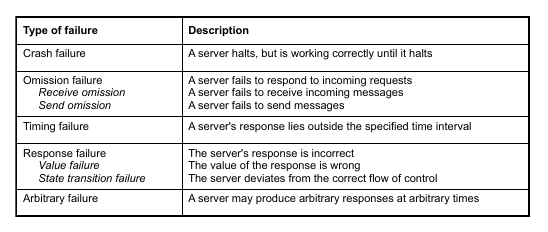
\includegraphics[width=0.8\textwidth]{failures.png}
   \caption{Failure models.}
   \label{fig:failures}
 \end{center}
\end{figure}
The different models of failure are shown in Figure \ref{fig:failures}. Typically fault tolerance mechanisms are assumed to provide safety against crash failures. Arbitrary failures may also be thought to be Byzantine failures where different behavior is observed at different times. These faults are typically very expensive to tolerate against.

\subsection{Redundancy}
\begin{figure}
\begin{center}
   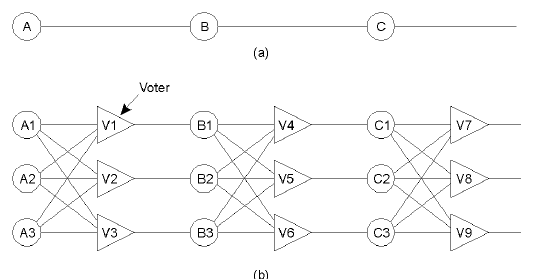
\includegraphics[width=0.8\textwidth]{redundancy.png}
   \caption{Failure masking by redundancy}
   \label{fig:redundancy}
 \end{center}
\end{figure}
Fault tolerance may be achieved by means of redundant computations and per stage voting. The circuit shown in Figure \ref{fig:redundancy} demonstrates this. Here each computation of the stages A, B and C is replicated and the results are aggregated by votes. This circuit is capable of tolerating one failure per stage of computation. If we try to deal with crash fault, we only need the replication degree to be 2, because we assume the node always produces the correct result if it's alive. We need the replication degree of 3 to deal with Byzantine fault.

  \textit{2019 QA\\
  Q: Why replicate the voter?\\
  A: Voters can fail. Replicate the voter makes the system more resilient.\\
  }

\section{Next Lecture introduction}
K-fault tolerant: the system can tolerate $k$ concurrent faults. This means we need $k + 1$ replications. However, for Byzantine failures, this not enough, because the remaining replica can produce garbage result. In this case, we need $3k$ or $3k+1$ components.

\subsection{Consensus and Byzantine Faults}

\begin{figure}
\begin{center}
   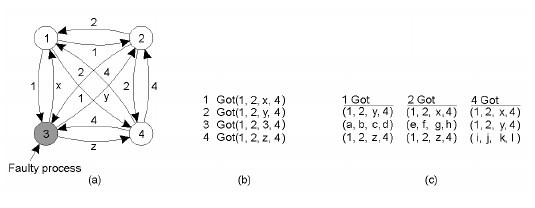
\includegraphics[width=0.8\textwidth]{byzantine.png}
   \caption{Recursive solution to Byzantine problem}
   \label{fig:byzantine}
\end{center}
\end{figure}

Byzantine faults can be modeled as a consensus problem (Byzantine Generals'
Problem) among nodes in presence of faulty processes assuming that a byzantine
node will force the system to \textit{not} reach consensus. A recursive solution
to the problem is provided in figure \ref{fig:byzantine}. In this, each node
collects information from all other nodes and sends it back to all others so
that each node now can see the view of the world from the perspective of other
nodes. By simple voting, each node can now either accept a single correct value or
can identify a byzantine failure.

In a system with $k$ such faults, $2k + 1$ total nodes are needed to only detect
that fault is present, while $3k + 1$ total nodes are needed to reach agreement,
despite the faults.

\end{document}
